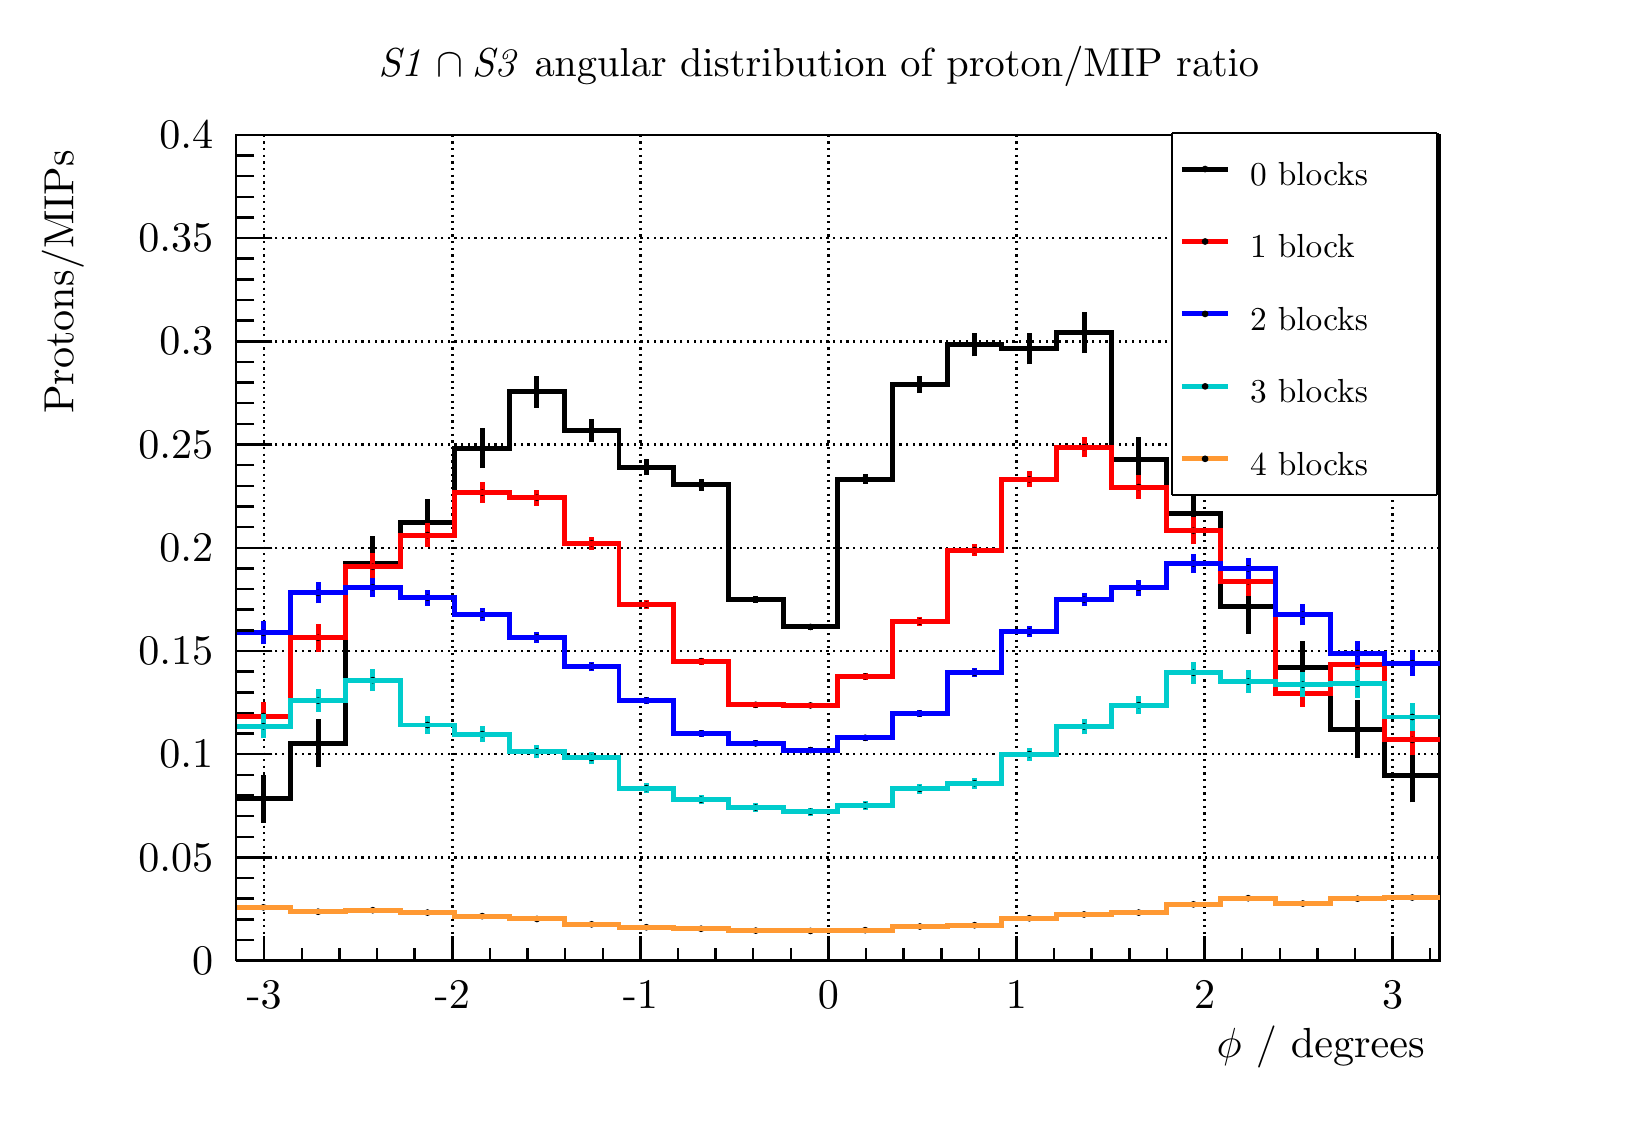
\begin{tikzpicture}
\pgfdeclareplotmark{cross} {
\pgfpathmoveto{\pgfpoint{-0.3\pgfplotmarksize}{\pgfplotmarksize}}
\pgfpathlineto{\pgfpoint{+0.3\pgfplotmarksize}{\pgfplotmarksize}}
\pgfpathlineto{\pgfpoint{+0.3\pgfplotmarksize}{0.3\pgfplotmarksize}}
\pgfpathlineto{\pgfpoint{+1\pgfplotmarksize}{0.3\pgfplotmarksize}}
\pgfpathlineto{\pgfpoint{+1\pgfplotmarksize}{-0.3\pgfplotmarksize}}
\pgfpathlineto{\pgfpoint{+0.3\pgfplotmarksize}{-0.3\pgfplotmarksize}}
\pgfpathlineto{\pgfpoint{+0.3\pgfplotmarksize}{-1.\pgfplotmarksize}}
\pgfpathlineto{\pgfpoint{-0.3\pgfplotmarksize}{-1.\pgfplotmarksize}}
\pgfpathlineto{\pgfpoint{-0.3\pgfplotmarksize}{-0.3\pgfplotmarksize}}
\pgfpathlineto{\pgfpoint{-1.\pgfplotmarksize}{-0.3\pgfplotmarksize}}
\pgfpathlineto{\pgfpoint{-1.\pgfplotmarksize}{0.3\pgfplotmarksize}}
\pgfpathlineto{\pgfpoint{-0.3\pgfplotmarksize}{0.3\pgfplotmarksize}}
\pgfpathclose
\pgfusepathqstroke
}
\pgfdeclareplotmark{cross*} {
\pgfpathmoveto{\pgfpoint{-0.3\pgfplotmarksize}{\pgfplotmarksize}}
\pgfpathlineto{\pgfpoint{+0.3\pgfplotmarksize}{\pgfplotmarksize}}
\pgfpathlineto{\pgfpoint{+0.3\pgfplotmarksize}{0.3\pgfplotmarksize}}
\pgfpathlineto{\pgfpoint{+1\pgfplotmarksize}{0.3\pgfplotmarksize}}
\pgfpathlineto{\pgfpoint{+1\pgfplotmarksize}{-0.3\pgfplotmarksize}}
\pgfpathlineto{\pgfpoint{+0.3\pgfplotmarksize}{-0.3\pgfplotmarksize}}
\pgfpathlineto{\pgfpoint{+0.3\pgfplotmarksize}{-1.\pgfplotmarksize}}
\pgfpathlineto{\pgfpoint{-0.3\pgfplotmarksize}{-1.\pgfplotmarksize}}
\pgfpathlineto{\pgfpoint{-0.3\pgfplotmarksize}{-0.3\pgfplotmarksize}}
\pgfpathlineto{\pgfpoint{-1.\pgfplotmarksize}{-0.3\pgfplotmarksize}}
\pgfpathlineto{\pgfpoint{-1.\pgfplotmarksize}{0.3\pgfplotmarksize}}
\pgfpathlineto{\pgfpoint{-0.3\pgfplotmarksize}{0.3\pgfplotmarksize}}
\pgfpathclose
\pgfusepathqfillstroke
}
\pgfdeclareplotmark{newstar} {
\pgfpathmoveto{\pgfqpoint{0pt}{\pgfplotmarksize}}
\pgfpathlineto{\pgfqpointpolar{44}{0.5\pgfplotmarksize}}
\pgfpathlineto{\pgfqpointpolar{18}{\pgfplotmarksize}}
\pgfpathlineto{\pgfqpointpolar{-20}{0.5\pgfplotmarksize}}
\pgfpathlineto{\pgfqpointpolar{-54}{\pgfplotmarksize}}
\pgfpathlineto{\pgfqpointpolar{-90}{0.5\pgfplotmarksize}}
\pgfpathlineto{\pgfqpointpolar{234}{\pgfplotmarksize}}
\pgfpathlineto{\pgfqpointpolar{198}{0.5\pgfplotmarksize}}
\pgfpathlineto{\pgfqpointpolar{162}{\pgfplotmarksize}}
\pgfpathlineto{\pgfqpointpolar{134}{0.5\pgfplotmarksize}}
\pgfpathclose
\pgfusepathqstroke
}
\pgfdeclareplotmark{newstar*} {
\pgfpathmoveto{\pgfqpoint{0pt}{\pgfplotmarksize}}
\pgfpathlineto{\pgfqpointpolar{44}{0.5\pgfplotmarksize}}
\pgfpathlineto{\pgfqpointpolar{18}{\pgfplotmarksize}}
\pgfpathlineto{\pgfqpointpolar{-20}{0.5\pgfplotmarksize}}
\pgfpathlineto{\pgfqpointpolar{-54}{\pgfplotmarksize}}
\pgfpathlineto{\pgfqpointpolar{-90}{0.5\pgfplotmarksize}}
\pgfpathlineto{\pgfqpointpolar{234}{\pgfplotmarksize}}
\pgfpathlineto{\pgfqpointpolar{198}{0.5\pgfplotmarksize}}
\pgfpathlineto{\pgfqpointpolar{162}{\pgfplotmarksize}}
\pgfpathlineto{\pgfqpointpolar{134}{0.5\pgfplotmarksize}}
\pgfpathclose
\pgfusepathqfillstroke
}
\definecolor{c}{rgb}{1,1,1};
\draw [color=c, fill=c] (0,0) rectangle (20,13.6286);
\draw [color=c, fill=c] (2.6,1.78641) rectangle (17.8857,12.2744);
\definecolor{c}{rgb}{0,0,0};
\draw [c,line width=0.9] (2.6,1.78641) -- (2.6,12.2744) -- (17.8857,12.2744) -- (17.8857,1.78641) -- (2.6,1.78641);
\definecolor{c}{rgb}{1,1,1};
\draw [color=c, fill=c] (2.6,1.78641) rectangle (17.8857,12.2744);
\definecolor{c}{rgb}{0,0,0};
\draw [c,line width=0.9] (2.6,1.78641) -- (2.6,12.2744) -- (17.8857,12.2744) -- (17.8857,1.78641) -- (2.6,1.78641);
\draw [c,line width=0.9] (2.6,1.78641) -- (17.8857,1.78641);
\draw [c,dash pattern=on 0.80pt off 1.60pt ,line width=0.9] (2.95826,12.2744) -- (2.95826,1.78641);
\draw [c,dash pattern=on 0.80pt off 1.60pt ,line width=0.9] (5.34665,12.2744) -- (5.34665,1.78641);
\draw [c,dash pattern=on 0.80pt off 1.60pt ,line width=0.9] (7.73504,12.2744) -- (7.73504,1.78641);
\draw [c,dash pattern=on 0.80pt off 1.60pt ,line width=0.9] (10.1234,12.2744) -- (10.1234,1.78641);
\draw [c,dash pattern=on 0.80pt off 1.60pt ,line width=0.9] (12.5118,12.2744) -- (12.5118,1.78641);
\draw [c,dash pattern=on 0.80pt off 1.60pt ,line width=0.9] (14.9002,12.2744) -- (14.9002,1.78641);
\draw [c,dash pattern=on 0.80pt off 1.60pt ,line width=0.9] (17.2886,12.2744) -- (17.2886,1.78641);
\draw [c,dash pattern=on 0.80pt off 1.60pt ,line width=0.9] (2.95826,12.2744) -- (2.95826,1.78641);
\draw [c,dash pattern=on 0.80pt off 1.60pt ,line width=0.9] (17.2886,12.2744) -- (17.2886,1.78641);
\draw [c,line width=0.9] (2.6,1.78641) -- (2.6,12.2744);
\draw [c,dash pattern=on 0.80pt off 1.60pt ,line width=0.9] (17.8857,1.78641) -- (2.6,1.78641);
\draw [c,dash pattern=on 0.80pt off 1.60pt ,line width=0.9] (17.8857,3.0974) -- (2.6,3.0974);
\draw [c,dash pattern=on 0.80pt off 1.60pt ,line width=0.9] (17.8857,4.4084) -- (2.6,4.4084);
\draw [c,dash pattern=on 0.80pt off 1.60pt ,line width=0.9] (17.8857,5.71939) -- (2.6,5.71939);
\draw [c,dash pattern=on 0.80pt off 1.60pt ,line width=0.9] (17.8857,7.03038) -- (2.6,7.03038);
\draw [c,dash pattern=on 0.80pt off 1.60pt ,line width=0.9] (17.8857,8.34138) -- (2.6,8.34138);
\draw [c,dash pattern=on 0.80pt off 1.60pt ,line width=0.9] (17.8857,9.65237) -- (2.6,9.65237);
\draw [c,dash pattern=on 0.80pt off 1.60pt ,line width=0.9] (17.8857,10.9634) -- (2.6,10.9634);
\draw [c,dash pattern=on 0.80pt off 1.60pt ,line width=0.9] (17.8857,12.2744) -- (2.6,12.2744);
\definecolor{c}{rgb}{0,0,0.6};
\draw [c,line width=0.9] (2.6,1.78641) -- (3.29481,1.78641) -- (3.29481,1.78641) -- (3.98961,1.78641) -- (3.98961,1.78641) -- (4.68442,1.78641) -- (4.68442,1.78641) -- (5.37922,1.78641) -- (5.37922,1.78641) -- (6.07403,1.78641) -- (6.07403,1.78641)
 -- (6.76883,1.78641) -- (6.76883,1.78641) -- (7.46364,1.78641) -- (7.46364,1.78641) -- (8.15844,1.78641) -- (8.15844,1.78641) -- (8.85325,1.78641) -- (8.85325,1.78641) -- (9.54805,1.78641) -- (9.54805,1.78641) -- (10.2429,1.78641) --
 (10.2429,1.78641) -- (10.9377,1.78641) -- (10.9377,1.78641) -- (11.6325,1.78641) -- (11.6325,1.78641) -- (12.3273,1.78641) -- (12.3273,1.78641) -- (13.0221,1.78641) -- (13.0221,1.78641) -- (13.7169,1.78641) -- (13.7169,1.78641) -- (14.4117,1.78641)
 -- (14.4117,1.78641) -- (15.1065,1.78641) -- (15.1065,1.78641) -- (15.8013,1.78641) -- (15.8013,1.78641) -- (16.4961,1.78641) -- (16.4961,1.78641) -- (17.1909,1.78641) -- (17.1909,1.78641) -- (17.8857,1.78641);
\definecolor{c}{rgb}{0,0,0};
\draw [c,line width=0.9] (2.6,1.78641) -- (17.8857,1.78641);
\draw [c,line width=0.9] (2.95826,2.09889) -- (2.95826,1.78641);
\draw [c,line width=0.9] (3.43594,1.94265) -- (3.43594,1.78641);
\draw [c,line width=0.9] (3.91362,1.94265) -- (3.91362,1.78641);
\draw [c,line width=0.9] (4.39129,1.94265) -- (4.39129,1.78641);
\draw [c,line width=0.9] (4.86897,1.94265) -- (4.86897,1.78641);
\draw [c,line width=0.9] (5.34665,2.09889) -- (5.34665,1.78641);
\draw [c,line width=0.9] (5.82433,1.94265) -- (5.82433,1.78641);
\draw [c,line width=0.9] (6.30201,1.94265) -- (6.30201,1.78641);
\draw [c,line width=0.9] (6.77969,1.94265) -- (6.77969,1.78641);
\draw [c,line width=0.9] (7.25737,1.94265) -- (7.25737,1.78641);
\draw [c,line width=0.9] (7.73504,2.09889) -- (7.73504,1.78641);
\draw [c,line width=0.9] (8.21272,1.94265) -- (8.21272,1.78641);
\draw [c,line width=0.9] (8.6904,1.94265) -- (8.6904,1.78641);
\draw [c,line width=0.9] (9.16808,1.94265) -- (9.16808,1.78641);
\draw [c,line width=0.9] (9.64576,1.94265) -- (9.64576,1.78641);
\draw [c,line width=0.9] (10.1234,2.09889) -- (10.1234,1.78641);
\draw [c,line width=0.9] (10.6011,1.94265) -- (10.6011,1.78641);
\draw [c,line width=0.9] (11.0788,1.94265) -- (11.0788,1.78641);
\draw [c,line width=0.9] (11.5565,1.94265) -- (11.5565,1.78641);
\draw [c,line width=0.9] (12.0342,1.94265) -- (12.0342,1.78641);
\draw [c,line width=0.9] (12.5118,2.09889) -- (12.5118,1.78641);
\draw [c,line width=0.9] (12.9895,1.94265) -- (12.9895,1.78641);
\draw [c,line width=0.9] (13.4672,1.94265) -- (13.4672,1.78641);
\draw [c,line width=0.9] (13.9449,1.94265) -- (13.9449,1.78641);
\draw [c,line width=0.9] (14.4225,1.94265) -- (14.4225,1.78641);
\draw [c,line width=0.9] (14.9002,2.09889) -- (14.9002,1.78641);
\draw [c,line width=0.9] (15.3779,1.94265) -- (15.3779,1.78641);
\draw [c,line width=0.9] (15.8556,1.94265) -- (15.8556,1.78641);
\draw [c,line width=0.9] (16.3333,1.94265) -- (16.3333,1.78641);
\draw [c,line width=0.9] (16.8109,1.94265) -- (16.8109,1.78641);
\draw [c,line width=0.9] (17.2886,2.09889) -- (17.2886,1.78641);
\draw [c,line width=0.9] (2.95826,2.09889) -- (2.95826,1.78641);
\draw [c,line width=0.9] (17.2886,2.09889) -- (17.2886,1.78641);
\draw [c,line width=0.9] (17.7663,1.94265) -- (17.7663,1.78641);
\draw [anchor=base] (2.95826,1.17312) node[scale=1.52295, color=c, rotate=0]{-3};
\draw [anchor=base] (5.34665,1.17312) node[scale=1.52295, color=c, rotate=0]{-2};
\draw [anchor=base] (7.73504,1.17312) node[scale=1.52295, color=c, rotate=0]{-1};
\draw [anchor=base] (10.1234,1.17312) node[scale=1.52295, color=c, rotate=0]{0};
\draw [anchor=base] (12.5118,1.17312) node[scale=1.52295, color=c, rotate=0]{1};
\draw [anchor=base] (14.9002,1.17312) node[scale=1.52295, color=c, rotate=0]{2};
\draw [anchor=base] (17.2886,1.17312) node[scale=1.52295, color=c, rotate=0]{3};
\draw [anchor= east] (17.8857,0.696123) node[scale=1.52295, color=c, rotate=0]{$\phi$ / degrees};
\draw [c,line width=0.9] (2.6,1.78641) -- (2.6,12.2744);
\draw [c,line width=0.9] (3.06173,1.78641) -- (2.6,1.78641);
\draw [c,line width=0.9] (2.83087,2.04861) -- (2.6,2.04861);
\draw [c,line width=0.9] (2.83087,2.31081) -- (2.6,2.31081);
\draw [c,line width=0.9] (2.83087,2.57301) -- (2.6,2.57301);
\draw [c,line width=0.9] (2.83087,2.8352) -- (2.6,2.8352);
\draw [c,line width=0.9] (3.06173,3.0974) -- (2.6,3.0974);
\draw [c,line width=0.9] (2.83087,3.3596) -- (2.6,3.3596);
\draw [c,line width=0.9] (2.83087,3.6218) -- (2.6,3.6218);
\draw [c,line width=0.9] (2.83087,3.884) -- (2.6,3.884);
\draw [c,line width=0.9] (2.83087,4.1462) -- (2.6,4.1462);
\draw [c,line width=0.9] (3.06173,4.4084) -- (2.6,4.4084);
\draw [c,line width=0.9] (2.83087,4.6706) -- (2.6,4.6706);
\draw [c,line width=0.9] (2.83087,4.93279) -- (2.6,4.93279);
\draw [c,line width=0.9] (2.83087,5.19499) -- (2.6,5.19499);
\draw [c,line width=0.9] (2.83087,5.45719) -- (2.6,5.45719);
\draw [c,line width=0.9] (3.06173,5.71939) -- (2.6,5.71939);
\draw [c,line width=0.9] (2.83087,5.98159) -- (2.6,5.98159);
\draw [c,line width=0.9] (2.83087,6.24379) -- (2.6,6.24379);
\draw [c,line width=0.9] (2.83087,6.50599) -- (2.6,6.50599);
\draw [c,line width=0.9] (2.83087,6.76819) -- (2.6,6.76819);
\draw [c,line width=0.9] (3.06173,7.03038) -- (2.6,7.03038);
\draw [c,line width=0.9] (2.83087,7.29258) -- (2.6,7.29258);
\draw [c,line width=0.9] (2.83087,7.55478) -- (2.6,7.55478);
\draw [c,line width=0.9] (2.83087,7.81698) -- (2.6,7.81698);
\draw [c,line width=0.9] (2.83087,8.07918) -- (2.6,8.07918);
\draw [c,line width=0.9] (3.06173,8.34138) -- (2.6,8.34138);
\draw [c,line width=0.9] (2.83087,8.60358) -- (2.6,8.60358);
\draw [c,line width=0.9] (2.83087,8.86578) -- (2.6,8.86578);
\draw [c,line width=0.9] (2.83087,9.12797) -- (2.6,9.12797);
\draw [c,line width=0.9] (2.83087,9.39017) -- (2.6,9.39017);
\draw [c,line width=0.9] (3.06173,9.65237) -- (2.6,9.65237);
\draw [c,line width=0.9] (2.83087,9.91457) -- (2.6,9.91457);
\draw [c,line width=0.9] (2.83087,10.1768) -- (2.6,10.1768);
\draw [c,line width=0.9] (2.83087,10.439) -- (2.6,10.439);
\draw [c,line width=0.9] (2.83087,10.7012) -- (2.6,10.7012);
\draw [c,line width=0.9] (3.06173,10.9634) -- (2.6,10.9634);
\draw [c,line width=0.9] (2.83087,11.2256) -- (2.6,11.2256);
\draw [c,line width=0.9] (2.83087,11.4878) -- (2.6,11.4878);
\draw [c,line width=0.9] (2.83087,11.75) -- (2.6,11.75);
\draw [c,line width=0.9] (2.83087,12.0122) -- (2.6,12.0122);
\draw [c,line width=0.9] (3.06173,12.2744) -- (2.6,12.2744);
\draw [anchor= east] (2.5,1.78641) node[scale=1.52295, color=c, rotate=0]{0};
\draw [anchor= east] (2.5,3.0974) node[scale=1.52295, color=c, rotate=0]{0.05};
\draw [anchor= east] (2.5,4.4084) node[scale=1.52295, color=c, rotate=0]{0.1};
\draw [anchor= east] (2.5,5.71939) node[scale=1.52295, color=c, rotate=0]{0.15};
\draw [anchor= east] (2.5,7.03038) node[scale=1.52295, color=c, rotate=0]{0.2};
\draw [anchor= east] (2.5,8.34138) node[scale=1.52295, color=c, rotate=0]{0.25};
\draw [anchor= east] (2.5,9.65237) node[scale=1.52295, color=c, rotate=0]{0.3};
\draw [anchor= east] (2.5,10.9634) node[scale=1.52295, color=c, rotate=0]{0.35};
\draw [anchor= east] (2.5,12.2744) node[scale=1.52295, color=c, rotate=0]{0.4};
\draw [anchor= east] (0.4,12.2744) node[scale=1.52295, color=c, rotate=90]{  Protons/MIPs};
\draw [c,line width=1.8] (2.9474,3.53935) -- (2.9474,3.84234);
\draw [c,line width=1.8] (2.9474,3.84234) -- (2.9474,4.14533);
\foreach \P in {(2.9474,3.84234)}{\draw[mark options={color=c,fill=c},mark size=2.402402pt,mark=*,mark size=1pt] plot coordinates {\P};}
\draw [c,line width=1.8] (3.64221,4.24112) -- (3.64221,4.54831);
\draw [c,line width=1.8] (3.64221,4.54831) -- (3.64221,4.8555);
\foreach \P in {(3.64221,4.54831)}{\draw[mark options={color=c,fill=c},mark size=2.402402pt,mark=*,mark size=1pt] plot coordinates {\P};}
\draw [c,line width=1.8] (4.33701,6.48887) -- (4.33701,6.8341);
\draw [c,line width=1.8] (4.33701,6.8341) -- (4.33701,7.17933);
\foreach \P in {(4.33701,6.8341)}{\draw[mark options={color=c,fill=c},mark size=2.402402pt,mark=*,mark size=1pt] plot coordinates {\P};}
\draw [c,line width=1.8] (5.03182,7.05025) -- (5.03182,7.34967);
\draw [c,line width=1.8] (5.03182,7.34967) -- (5.03182,7.64909);
\foreach \P in {(5.03182,7.34967)}{\draw[mark options={color=c,fill=c},mark size=2.402402pt,mark=*,mark size=1pt] plot coordinates {\P};}
\draw [c,line width=1.8] (5.72662,8.04159) -- (5.72662,8.29382);
\draw [c,line width=1.8] (5.72662,8.29382) -- (5.72662,8.54604);
\foreach \P in {(5.72662,8.29382)}{\draw[mark options={color=c,fill=c},mark size=2.402402pt,mark=*,mark size=1pt] plot coordinates {\P};}
\draw [c,line width=1.8] (6.42143,8.80975) -- (6.42143,9.01057);
\draw [c,line width=1.8] (6.42143,9.01057) -- (6.42143,9.21139);
\foreach \P in {(6.42143,9.01057)}{\draw[mark options={color=c,fill=c},mark size=2.402402pt,mark=*,mark size=1pt] plot coordinates {\P};}
\draw [c,line width=1.8] (7.11623,8.37439) -- (7.11623,8.52183);
\draw [c,line width=1.8] (7.11623,8.52183) -- (7.11623,8.66927);
\foreach \P in {(7.11623,8.52183)}{\draw[mark options={color=c,fill=c},mark size=2.402402pt,mark=*,mark size=1pt] plot coordinates {\P};}
\draw [c,line width=1.8] (7.81104,7.9511) -- (7.81104,8.05321);
\draw [c,line width=1.8] (7.81104,8.05321) -- (7.81104,8.15533);
\foreach \P in {(7.81104,8.05321)}{\draw[mark options={color=c,fill=c},mark size=2.402402pt,mark=*,mark size=1pt] plot coordinates {\P};}
\draw [c,line width=1.8] (8.50584,7.75621) -- (8.50584,7.8287);
\draw [c,line width=1.8] (8.50584,7.8287) -- (8.50584,7.90119);
\foreach \P in {(8.50584,7.8287)}{\draw[mark options={color=c,fill=c},mark size=2.402402pt,mark=*,mark size=1pt] plot coordinates {\P};}
\draw [c,line width=1.8] (9.20065,6.33291) -- (9.20065,6.37243);
\draw [c,line width=1.8] (9.20065,6.37243) -- (9.20065,6.41195);
\foreach \P in {(9.20065,6.37243)}{\draw[mark options={color=c,fill=c},mark size=2.402402pt,mark=*,mark size=1pt] plot coordinates {\P};}
\draw [c,line width=1.8] (9.89545,5.9895) -- (9.89545,6.02497);
\draw [c,line width=1.8] (9.89545,6.02497) -- (9.89545,6.06044);
\foreach \P in {(9.89545,6.02497)}{\draw[mark options={color=c,fill=c},mark size=2.402402pt,mark=*,mark size=1pt] plot coordinates {\P};}
\draw [c,line width=1.8] (10.5903,7.84021) -- (10.5903,7.90312);
\draw [c,line width=1.8] (10.5903,7.90312) -- (10.5903,7.96603);
\foreach \P in {(10.5903,7.90312)}{\draw[mark options={color=c,fill=c},mark size=2.402402pt,mark=*,mark size=1pt] plot coordinates {\P};}
\draw [c,line width=1.8] (11.2851,8.99555) -- (11.2851,9.10057);
\draw [c,line width=1.8] (11.2851,9.10057) -- (11.2851,9.20559);
\foreach \P in {(11.2851,9.10057)}{\draw[mark options={color=c,fill=c},mark size=2.402402pt,mark=*,mark size=1pt] plot coordinates {\P};}
\draw [c,line width=1.8] (11.9799,9.46091) -- (11.9799,9.60828);
\draw [c,line width=1.8] (11.9799,9.60828) -- (11.9799,9.75566);
\foreach \P in {(11.9799,9.60828)}{\draw[mark options={color=c,fill=c},mark size=2.402402pt,mark=*,mark size=1pt] plot coordinates {\P};}
\draw [c,line width=1.8] (12.6747,9.35796) -- (12.6747,9.5602);
\draw [c,line width=1.8] (12.6747,9.5602) -- (12.6747,9.76245);
\foreach \P in {(12.6747,9.5602)}{\draw[mark options={color=c,fill=c},mark size=2.402402pt,mark=*,mark size=1pt] plot coordinates {\P};}
\draw [c,line width=1.8] (13.3695,9.50201) -- (13.3695,9.76182);
\draw [c,line width=1.8] (13.3695,9.76182) -- (13.3695,10.0216);
\foreach \P in {(13.3695,9.76182)}{\draw[mark options={color=c,fill=c},mark size=2.402402pt,mark=*,mark size=1pt] plot coordinates {\P};}
\draw [c,line width=1.8] (14.0643,7.8623) -- (14.0643,8.14905);
\draw [c,line width=1.8] (14.0643,8.14905) -- (14.0643,8.43581);
\foreach \P in {(14.0643,8.14905)}{\draw[mark options={color=c,fill=c},mark size=2.402402pt,mark=*,mark size=1pt] plot coordinates {\P};}
\draw [c,line width=1.8] (14.7591,7.12067) -- (14.7591,7.46209);
\draw [c,line width=1.8] (14.7591,7.46209) -- (14.7591,7.80352);
\foreach \P in {(14.7591,7.46209)}{\draw[mark options={color=c,fill=c},mark size=2.402402pt,mark=*,mark size=1pt] plot coordinates {\P};}
\draw [c,line width=1.8] (15.4539,5.94094) -- (15.4539,6.28075);
\draw [c,line width=1.8] (15.4539,6.28075) -- (15.4539,6.62055);
\foreach \P in {(15.4539,6.28075)}{\draw[mark options={color=c,fill=c},mark size=2.402402pt,mark=*,mark size=1pt] plot coordinates {\P};}
\draw [c,line width=1.8] (16.1487,5.16867) -- (16.1487,5.50527);
\draw [c,line width=1.8] (16.1487,5.50527) -- (16.1487,5.84187);
\foreach \P in {(16.1487,5.50527)}{\draw[mark options={color=c,fill=c},mark size=2.402402pt,mark=*,mark size=1pt] plot coordinates {\P};}
\draw [c,line width=1.8] (16.8435,4.36122) -- (16.8435,4.72749);
\draw [c,line width=1.8] (16.8435,4.72749) -- (16.8435,5.09375);
\foreach \P in {(16.8435,4.72749)}{\draw[mark options={color=c,fill=c},mark size=2.402402pt,mark=*,mark size=1pt] plot coordinates {\P};}
\draw [c,line width=1.8] (17.5383,3.7966) -- (17.5383,4.13675);
\draw [c,line width=1.8] (17.5383,4.13675) -- (17.5383,4.47691);
\foreach \P in {(17.5383,4.13675)}{\draw[mark options={color=c,fill=c},mark size=2.402402pt,mark=*,mark size=1pt] plot coordinates {\P};}
\draw [c,line width=1.8] (2.6,3.84234) -- (3.29481,3.84234) -- (3.29481,4.54831) -- (3.98961,4.54831) -- (3.98961,6.8341) -- (4.68442,6.8341) -- (4.68442,7.34967) -- (5.37922,7.34967) -- (5.37922,8.29382) -- (6.07403,8.29382) -- (6.07403,9.01057) --
 (6.76883,9.01057) -- (6.76883,8.52183) -- (7.46364,8.52183) -- (7.46364,8.05321) -- (8.15844,8.05321) -- (8.15844,7.8287) -- (8.85325,7.8287) -- (8.85325,6.37243) -- (9.54805,6.37243) -- (9.54805,6.02497) -- (10.2429,6.02497) -- (10.2429,7.90312) --
 (10.9377,7.90312) -- (10.9377,9.10057) -- (11.6325,9.10057) -- (11.6325,9.60828) -- (12.3273,9.60828) -- (12.3273,9.5602) -- (13.0221,9.5602) -- (13.0221,9.76182) -- (13.7169,9.76182) -- (13.7169,8.14905) -- (14.4117,8.14905) -- (14.4117,7.46209) --
 (15.1065,7.46209) -- (15.1065,6.28075) -- (15.8013,6.28075) -- (15.8013,5.50527) -- (16.4961,5.50527) -- (16.4961,4.72749) -- (17.1909,4.72749) -- (17.1909,4.13675) -- (17.8857,4.13675);
\definecolor{c}{rgb}{1,0,0};
\draw [c,line width=1.8] (2.9474,4.70943) -- (2.9474,4.89348);
\draw [c,line width=1.8] (2.9474,4.89348) -- (2.9474,5.07754);
\definecolor{c}{rgb}{0,0,0};
\foreach \P in {(2.9474,4.89348)}{\draw[mark options={color=c,fill=c},mark size=2.402402pt,mark=*,mark size=1pt] plot coordinates {\P};}
\definecolor{c}{rgb}{1,0,0};
\draw [c,line width=1.8] (3.64221,5.70749) -- (3.64221,5.8873);
\draw [c,line width=1.8] (3.64221,5.8873) -- (3.64221,6.06711);
\definecolor{c}{rgb}{0,0,0};
\foreach \P in {(3.64221,5.8873)}{\draw[mark options={color=c,fill=c},mark size=2.402402pt,mark=*,mark size=1pt] plot coordinates {\P};}
\definecolor{c}{rgb}{1,0,0};
\draw [c,line width=1.8] (4.33701,6.61434) -- (4.33701,6.78897);
\draw [c,line width=1.8] (4.33701,6.78897) -- (4.33701,6.96361);
\definecolor{c}{rgb}{0,0,0};
\foreach \P in {(4.33701,6.78897)}{\draw[mark options={color=c,fill=c},mark size=2.402402pt,mark=*,mark size=1pt] plot coordinates {\P};}
\definecolor{c}{rgb}{1,0,0};
\draw [c,line width=1.8] (5.03182,7.0415) -- (5.03182,7.19119);
\draw [c,line width=1.8] (5.03182,7.19119) -- (5.03182,7.34088);
\definecolor{c}{rgb}{0,0,0};
\foreach \P in {(5.03182,7.19119)}{\draw[mark options={color=c,fill=c},mark size=2.402402pt,mark=*,mark size=1pt] plot coordinates {\P};}
\definecolor{c}{rgb}{1,0,0};
\draw [c,line width=1.8] (5.72662,7.60056) -- (5.72662,7.73125);
\draw [c,line width=1.8] (5.72662,7.73125) -- (5.72662,7.86195);
\definecolor{c}{rgb}{0,0,0};
\foreach \P in {(5.72662,7.73125)}{\draw[mark options={color=c,fill=c},mark size=2.402402pt,mark=*,mark size=1pt] plot coordinates {\P};}
\definecolor{c}{rgb}{1,0,0};
\draw [c,line width=1.8] (6.42143,7.56324) -- (6.42143,7.66658);
\draw [c,line width=1.8] (6.42143,7.66658) -- (6.42143,7.76992);
\definecolor{c}{rgb}{0,0,0};
\foreach \P in {(6.42143,7.66658)}{\draw[mark options={color=c,fill=c},mark size=2.402402pt,mark=*,mark size=1pt] plot coordinates {\P};}
\definecolor{c}{rgb}{1,0,0};
\draw [c,line width=1.8] (7.11623,7.00825) -- (7.11623,7.08744);
\draw [c,line width=1.8] (7.11623,7.08744) -- (7.11623,7.16663);
\definecolor{c}{rgb}{0,0,0};
\foreach \P in {(7.11623,7.08744)}{\draw[mark options={color=c,fill=c},mark size=2.402402pt,mark=*,mark size=1pt] plot coordinates {\P};}
\definecolor{c}{rgb}{1,0,0};
\draw [c,line width=1.8] (7.81104,6.25066) -- (7.81104,6.30821);
\draw [c,line width=1.8] (7.81104,6.30821) -- (7.81104,6.36576);
\definecolor{c}{rgb}{0,0,0};
\foreach \P in {(7.81104,6.30821)}{\draw[mark options={color=c,fill=c},mark size=2.402402pt,mark=*,mark size=1pt] plot coordinates {\P};}
\definecolor{c}{rgb}{1,0,0};
\draw [c,line width=1.8] (8.50584,5.54487) -- (8.50584,5.59015);
\draw [c,line width=1.8] (8.50584,5.59015) -- (8.50584,5.63542);
\definecolor{c}{rgb}{0,0,0};
\foreach \P in {(8.50584,5.59015)}{\draw[mark options={color=c,fill=c},mark size=2.402402pt,mark=*,mark size=1pt] plot coordinates {\P};}
\definecolor{c}{rgb}{1,0,0};
\draw [c,line width=1.8] (9.20065,4.99986) -- (9.20065,5.03632);
\draw [c,line width=1.8] (9.20065,5.03632) -- (9.20065,5.07279);
\definecolor{c}{rgb}{0,0,0};
\foreach \P in {(9.20065,5.03632)}{\draw[mark options={color=c,fill=c},mark size=2.402402pt,mark=*,mark size=1pt] plot coordinates {\P};}
\definecolor{c}{rgb}{1,0,0};
\draw [c,line width=1.8] (9.89545,4.99189) -- (9.89545,5.02837);
\draw [c,line width=1.8] (9.89545,5.02837) -- (9.89545,5.06484);
\definecolor{c}{rgb}{0,0,0};
\foreach \P in {(9.89545,5.02837)}{\draw[mark options={color=c,fill=c},mark size=2.402402pt,mark=*,mark size=1pt] plot coordinates {\P};}
\definecolor{c}{rgb}{1,0,0};
\draw [c,line width=1.8] (10.5903,5.35598) -- (10.5903,5.39691);
\draw [c,line width=1.8] (10.5903,5.39691) -- (10.5903,5.43783);
\definecolor{c}{rgb}{0,0,0};
\foreach \P in {(10.5903,5.39691)}{\draw[mark options={color=c,fill=c},mark size=2.402402pt,mark=*,mark size=1pt] plot coordinates {\P};}
\definecolor{c}{rgb}{1,0,0};
\draw [c,line width=1.8] (11.2851,6.04002) -- (11.2851,6.09306);
\draw [c,line width=1.8] (11.2851,6.09306) -- (11.2851,6.1461);
\definecolor{c}{rgb}{0,0,0};
\foreach \P in {(11.2851,6.09306)}{\draw[mark options={color=c,fill=c},mark size=2.402402pt,mark=*,mark size=1pt] plot coordinates {\P};}
\definecolor{c}{rgb}{1,0,0};
\draw [c,line width=1.8] (11.9799,6.93102) -- (11.9799,7.00185);
\draw [c,line width=1.8] (11.9799,7.00185) -- (11.9799,7.07268);
\definecolor{c}{rgb}{0,0,0};
\foreach \P in {(11.9799,7.00185)}{\draw[mark options={color=c,fill=c},mark size=2.402402pt,mark=*,mark size=1pt] plot coordinates {\P};}
\definecolor{c}{rgb}{1,0,0};
\draw [c,line width=1.8] (12.6747,7.79861) -- (12.6747,7.899);
\draw [c,line width=1.8] (12.6747,7.899) -- (12.6747,7.9994);
\definecolor{c}{rgb}{0,0,0};
\foreach \P in {(12.6747,7.899)}{\draw[mark options={color=c,fill=c},mark size=2.402402pt,mark=*,mark size=1pt] plot coordinates {\P};}
\definecolor{c}{rgb}{1,0,0};
\draw [c,line width=1.8] (13.3695,8.1816) -- (13.3695,8.30978);
\draw [c,line width=1.8] (13.3695,8.30978) -- (13.3695,8.43797);
\definecolor{c}{rgb}{0,0,0};
\foreach \P in {(13.3695,8.30978)}{\draw[mark options={color=c,fill=c},mark size=2.402402pt,mark=*,mark size=1pt] plot coordinates {\P};}
\definecolor{c}{rgb}{1,0,0};
\draw [c,line width=1.8] (14.0643,7.6524) -- (14.0643,7.80143);
\draw [c,line width=1.8] (14.0643,7.80143) -- (14.0643,7.95045);
\definecolor{c}{rgb}{0,0,0};
\foreach \P in {(14.0643,7.80143)}{\draw[mark options={color=c,fill=c},mark size=2.402402pt,mark=*,mark size=1pt] plot coordinates {\P};}
\definecolor{c}{rgb}{1,0,0};
\draw [c,line width=1.8] (14.7591,7.07351) -- (14.7591,7.24762);
\draw [c,line width=1.8] (14.7591,7.24762) -- (14.7591,7.42173);
\definecolor{c}{rgb}{0,0,0};
\foreach \P in {(14.7591,7.24762)}{\draw[mark options={color=c,fill=c},mark size=2.402402pt,mark=*,mark size=1pt] plot coordinates {\P};}
\definecolor{c}{rgb}{1,0,0};
\draw [c,line width=1.8] (15.4539,6.42259) -- (15.4539,6.60472);
\draw [c,line width=1.8] (15.4539,6.60472) -- (15.4539,6.78686);
\definecolor{c}{rgb}{0,0,0};
\foreach \P in {(15.4539,6.60472)}{\draw[mark options={color=c,fill=c},mark size=2.402402pt,mark=*,mark size=1pt] plot coordinates {\P};}
\definecolor{c}{rgb}{1,0,0};
\draw [c,line width=1.8] (16.1487,5.01154) -- (16.1487,5.18261);
\draw [c,line width=1.8] (16.1487,5.18261) -- (16.1487,5.35368);
\definecolor{c}{rgb}{0,0,0};
\foreach \P in {(16.1487,5.18261)}{\draw[mark options={color=c,fill=c},mark size=2.402402pt,mark=*,mark size=1pt] plot coordinates {\P};}
\definecolor{c}{rgb}{1,0,0};
\draw [c,line width=1.8] (16.8435,5.33667) -- (16.8435,5.54473);
\draw [c,line width=1.8] (16.8435,5.54473) -- (16.8435,5.75279);
\definecolor{c}{rgb}{0,0,0};
\foreach \P in {(16.8435,5.54473)}{\draw[mark options={color=c,fill=c},mark size=2.402402pt,mark=*,mark size=1pt] plot coordinates {\P};}
\definecolor{c}{rgb}{1,0,0};
\draw [c,line width=1.8] (17.5383,4.39276) -- (17.5383,4.59024);
\draw [c,line width=1.8] (17.5383,4.59024) -- (17.5383,4.78771);
\definecolor{c}{rgb}{0,0,0};
\foreach \P in {(17.5383,4.59024)}{\draw[mark options={color=c,fill=c},mark size=2.402402pt,mark=*,mark size=1pt] plot coordinates {\P};}
\definecolor{c}{rgb}{1,0,0};
\draw [c,line width=1.8] (2.6,4.89348) -- (3.29481,4.89348) -- (3.29481,5.8873) -- (3.98961,5.8873) -- (3.98961,6.78897) -- (4.68442,6.78897) -- (4.68442,7.19119) -- (5.37922,7.19119) -- (5.37922,7.73125) -- (6.07403,7.73125) -- (6.07403,7.66658) --
 (6.76883,7.66658) -- (6.76883,7.08744) -- (7.46364,7.08744) -- (7.46364,6.30821) -- (8.15844,6.30821) -- (8.15844,5.59015) -- (8.85325,5.59015) -- (8.85325,5.03632) -- (9.54805,5.03632) -- (9.54805,5.02837) -- (10.2429,5.02837) -- (10.2429,5.39691)
 -- (10.9377,5.39691) -- (10.9377,6.09306) -- (11.6325,6.09306) -- (11.6325,7.00185) -- (12.3273,7.00185) -- (12.3273,7.899) -- (13.0221,7.899) -- (13.0221,8.30978) -- (13.7169,8.30978) -- (13.7169,7.80143) -- (14.4117,7.80143) -- (14.4117,7.24762)
 -- (15.1065,7.24762) -- (15.1065,6.60472) -- (15.8013,6.60472) -- (15.8013,5.18261) -- (16.4961,5.18261) -- (16.4961,5.54473) -- (17.1909,5.54473) -- (17.1909,4.59024) -- (17.8857,4.59024);
\definecolor{c}{rgb}{0,0,1};
\draw [c,line width=1.8] (2.9474,5.80356) -- (2.9474,5.94975);
\draw [c,line width=1.8] (2.9474,5.94975) -- (2.9474,6.09593);
\definecolor{c}{rgb}{0,0,0};
\foreach \P in {(2.9474,5.94975)}{\draw[mark options={color=c,fill=c},mark size=2.402402pt,mark=*,mark size=1pt] plot coordinates {\P};}
\definecolor{c}{rgb}{0,0,1};
\draw [c,line width=1.8] (3.64221,6.32429) -- (3.64221,6.45775);
\draw [c,line width=1.8] (3.64221,6.45775) -- (3.64221,6.59121);
\definecolor{c}{rgb}{0,0,0};
\foreach \P in {(3.64221,6.45775)}{\draw[mark options={color=c,fill=c},mark size=2.402402pt,mark=*,mark size=1pt] plot coordinates {\P};}
\definecolor{c}{rgb}{0,0,1};
\draw [c,line width=1.8] (4.33701,6.40743) -- (4.33701,6.52913);
\draw [c,line width=1.8] (4.33701,6.52913) -- (4.33701,6.65083);
\definecolor{c}{rgb}{0,0,0};
\foreach \P in {(4.33701,6.52913)}{\draw[mark options={color=c,fill=c},mark size=2.402402pt,mark=*,mark size=1pt] plot coordinates {\P};}
\definecolor{c}{rgb}{0,0,1};
\draw [c,line width=1.8] (5.03182,6.29377) -- (5.03182,6.39613);
\draw [c,line width=1.8] (5.03182,6.39613) -- (5.03182,6.49849);
\definecolor{c}{rgb}{0,0,0};
\foreach \P in {(5.03182,6.39613)}{\draw[mark options={color=c,fill=c},mark size=2.402402pt,mark=*,mark size=1pt] plot coordinates {\P};}
\definecolor{c}{rgb}{0,0,1};
\draw [c,line width=1.8] (5.72662,6.0959) -- (5.72662,6.18284);
\draw [c,line width=1.8] (5.72662,6.18284) -- (5.72662,6.26979);
\definecolor{c}{rgb}{0,0,0};
\foreach \P in {(5.72662,6.18284)}{\draw[mark options={color=c,fill=c},mark size=2.402402pt,mark=*,mark size=1pt] plot coordinates {\P};}
\definecolor{c}{rgb}{0,0,1};
\draw [c,line width=1.8] (6.42143,5.82197) -- (6.42143,5.8941);
\draw [c,line width=1.8] (6.42143,5.8941) -- (6.42143,5.96623);
\definecolor{c}{rgb}{0,0,0};
\foreach \P in {(6.42143,5.8941)}{\draw[mark options={color=c,fill=c},mark size=2.402402pt,mark=*,mark size=1pt] plot coordinates {\P};}
\definecolor{c}{rgb}{0,0,1};
\draw [c,line width=1.8] (7.11623,5.46105) -- (7.11623,5.52162);
\draw [c,line width=1.8] (7.11623,5.52162) -- (7.11623,5.5822);
\definecolor{c}{rgb}{0,0,0};
\foreach \P in {(7.11623,5.52162)}{\draw[mark options={color=c,fill=c},mark size=2.402402pt,mark=*,mark size=1pt] plot coordinates {\P};}
\definecolor{c}{rgb}{0,0,1};
\draw [c,line width=1.8] (7.81104,5.04345) -- (7.81104,5.09233);
\draw [c,line width=1.8] (7.81104,5.09233) -- (7.81104,5.14121);
\definecolor{c}{rgb}{0,0,0};
\foreach \P in {(7.81104,5.09233)}{\draw[mark options={color=c,fill=c},mark size=2.402402pt,mark=*,mark size=1pt] plot coordinates {\P};}
\definecolor{c}{rgb}{0,0,1};
\draw [c,line width=1.8] (8.50584,4.63128) -- (8.50584,4.67322);
\draw [c,line width=1.8] (8.50584,4.67322) -- (8.50584,4.71517);
\definecolor{c}{rgb}{0,0,0};
\foreach \P in {(8.50584,4.67322)}{\draw[mark options={color=c,fill=c},mark size=2.402402pt,mark=*,mark size=1pt] plot coordinates {\P};}
\definecolor{c}{rgb}{0,0,1};
\draw [c,line width=1.8] (9.20065,4.508) -- (9.20065,4.5457);
\draw [c,line width=1.8] (9.20065,4.5457) -- (9.20065,4.58341);
\definecolor{c}{rgb}{0,0,0};
\foreach \P in {(9.20065,4.5457)}{\draw[mark options={color=c,fill=c},mark size=2.402402pt,mark=*,mark size=1pt] plot coordinates {\P};}
\definecolor{c}{rgb}{0,0,1};
\draw [c,line width=1.8] (9.89545,4.42281) -- (9.89545,4.46059);
\draw [c,line width=1.8] (9.89545,4.46059) -- (9.89545,4.49836);
\definecolor{c}{rgb}{0,0,0};
\foreach \P in {(9.89545,4.46059)}{\draw[mark options={color=c,fill=c},mark size=2.402402pt,mark=*,mark size=1pt] plot coordinates {\P};}
\definecolor{c}{rgb}{0,0,1};
\draw [c,line width=1.8] (10.5903,4.57747) -- (10.5903,4.61724);
\draw [c,line width=1.8] (10.5903,4.61724) -- (10.5903,4.65702);
\definecolor{c}{rgb}{0,0,0};
\foreach \P in {(10.5903,4.61724)}{\draw[mark options={color=c,fill=c},mark size=2.402402pt,mark=*,mark size=1pt] plot coordinates {\P};}
\definecolor{c}{rgb}{0,0,1};
\draw [c,line width=1.8] (11.2851,4.87808) -- (11.2851,4.92461);
\draw [c,line width=1.8] (11.2851,4.92461) -- (11.2851,4.97114);
\definecolor{c}{rgb}{0,0,0};
\foreach \P in {(11.2851,4.92461)}{\draw[mark options={color=c,fill=c},mark size=2.402402pt,mark=*,mark size=1pt] plot coordinates {\P};}
\definecolor{c}{rgb}{0,0,1};
\draw [c,line width=1.8] (11.9799,5.38665) -- (11.9799,5.44283);
\draw [c,line width=1.8] (11.9799,5.44283) -- (11.9799,5.49901);
\definecolor{c}{rgb}{0,0,0};
\foreach \P in {(11.9799,5.44283)}{\draw[mark options={color=c,fill=c},mark size=2.402402pt,mark=*,mark size=1pt] plot coordinates {\P};}
\definecolor{c}{rgb}{0,0,1};
\draw [c,line width=1.8] (12.6747,5.89507) -- (12.6747,5.967);
\draw [c,line width=1.8] (12.6747,5.967) -- (12.6747,6.03894);
\definecolor{c}{rgb}{0,0,0};
\foreach \P in {(12.6747,5.967)}{\draw[mark options={color=c,fill=c},mark size=2.402402pt,mark=*,mark size=1pt] plot coordinates {\P};}
\definecolor{c}{rgb}{0,0,1};
\draw [c,line width=1.8] (13.3695,6.28448) -- (13.3695,6.37204);
\draw [c,line width=1.8] (13.3695,6.37204) -- (13.3695,6.45959);
\definecolor{c}{rgb}{0,0,0};
\foreach \P in {(13.3695,6.37204)}{\draw[mark options={color=c,fill=c},mark size=2.402402pt,mark=*,mark size=1pt] plot coordinates {\P};}
\definecolor{c}{rgb}{0,0,1};
\draw [c,line width=1.8] (14.0643,6.42072) -- (14.0643,6.52104);
\draw [c,line width=1.8] (14.0643,6.52104) -- (14.0643,6.62135);
\definecolor{c}{rgb}{0,0,0};
\foreach \P in {(14.0643,6.52104)}{\draw[mark options={color=c,fill=c},mark size=2.402402pt,mark=*,mark size=1pt] plot coordinates {\P};}
\definecolor{c}{rgb}{0,0,1};
\draw [c,line width=1.8] (14.7591,6.70949) -- (14.7591,6.82981);
\draw [c,line width=1.8] (14.7591,6.82981) -- (14.7591,6.95012);
\definecolor{c}{rgb}{0,0,0};
\foreach \P in {(14.7591,6.82981)}{\draw[mark options={color=c,fill=c},mark size=2.402402pt,mark=*,mark size=1pt] plot coordinates {\P};}
\definecolor{c}{rgb}{0,0,1};
\draw [c,line width=1.8] (15.4539,6.63578) -- (15.4539,6.76781);
\draw [c,line width=1.8] (15.4539,6.76781) -- (15.4539,6.89983);
\definecolor{c}{rgb}{0,0,0};
\foreach \P in {(15.4539,6.76781)}{\draw[mark options={color=c,fill=c},mark size=2.402402pt,mark=*,mark size=1pt] plot coordinates {\P};}
\definecolor{c}{rgb}{0,0,1};
\draw [c,line width=1.8] (16.1487,6.04474) -- (16.1487,6.18175);
\draw [c,line width=1.8] (16.1487,6.18175) -- (16.1487,6.31876);
\definecolor{c}{rgb}{0,0,0};
\foreach \P in {(16.1487,6.18175)}{\draw[mark options={color=c,fill=c},mark size=2.402402pt,mark=*,mark size=1pt] plot coordinates {\P};}
\definecolor{c}{rgb}{0,0,1};
\draw [c,line width=1.8] (16.8435,5.54467) -- (16.8435,5.69354);
\draw [c,line width=1.8] (16.8435,5.69354) -- (16.8435,5.84241);
\definecolor{c}{rgb}{0,0,0};
\foreach \P in {(16.8435,5.69354)}{\draw[mark options={color=c,fill=c},mark size=2.402402pt,mark=*,mark size=1pt] plot coordinates {\P};}
\definecolor{c}{rgb}{0,0,1};
\draw [c,line width=1.8] (17.5383,5.40572) -- (17.5383,5.56626);
\draw [c,line width=1.8] (17.5383,5.56626) -- (17.5383,5.72679);
\definecolor{c}{rgb}{0,0,0};
\foreach \P in {(17.5383,5.56626)}{\draw[mark options={color=c,fill=c},mark size=2.402402pt,mark=*,mark size=1pt] plot coordinates {\P};}
\definecolor{c}{rgb}{0,0,1};
\draw [c,line width=1.8] (2.6,5.94975) -- (3.29481,5.94975) -- (3.29481,6.45775) -- (3.98961,6.45775) -- (3.98961,6.52913) -- (4.68442,6.52913) -- (4.68442,6.39613) -- (5.37922,6.39613) -- (5.37922,6.18284) -- (6.07403,6.18284) -- (6.07403,5.8941) --
 (6.76883,5.8941) -- (6.76883,5.52162) -- (7.46364,5.52162) -- (7.46364,5.09233) -- (8.15844,5.09233) -- (8.15844,4.67322) -- (8.85325,4.67322) -- (8.85325,4.5457) -- (9.54805,4.5457) -- (9.54805,4.46059) -- (10.2429,4.46059) -- (10.2429,4.61724) --
 (10.9377,4.61724) -- (10.9377,4.92461) -- (11.6325,4.92461) -- (11.6325,5.44283) -- (12.3273,5.44283) -- (12.3273,5.967) -- (13.0221,5.967) -- (13.0221,6.37204) -- (13.7169,6.37204) -- (13.7169,6.52104) -- (14.4117,6.52104) -- (14.4117,6.82981) --
 (15.1065,6.82981) -- (15.1065,6.76781) -- (15.8013,6.76781) -- (15.8013,6.18175) -- (16.4961,6.18175) -- (16.4961,5.69354) -- (17.1909,5.69354) -- (17.1909,5.56626) -- (17.8857,5.56626);
\definecolor{c}{rgb}{0,0.8,0.8};
\draw [c,line width=1.8] (2.9474,4.61284) -- (2.9474,4.76381);
\draw [c,line width=1.8] (2.9474,4.76381) -- (2.9474,4.91478);
\definecolor{c}{rgb}{0,0,0};
\foreach \P in {(2.9474,4.76381)}{\draw[mark options={color=c,fill=c},mark size=2.402402pt,mark=*,mark size=1pt] plot coordinates {\P};}
\definecolor{c}{rgb}{0,0.8,0.8};
\draw [c,line width=1.8] (3.64221,4.94708) -- (3.64221,5.08907);
\draw [c,line width=1.8] (3.64221,5.08907) -- (3.64221,5.23106);
\definecolor{c}{rgb}{0,0,0};
\foreach \P in {(3.64221,5.08907)}{\draw[mark options={color=c,fill=c},mark size=2.402402pt,mark=*,mark size=1pt] plot coordinates {\P};}
\definecolor{c}{rgb}{0,0.8,0.8};
\draw [c,line width=1.8] (4.33701,5.21061) -- (4.33701,5.34923);
\draw [c,line width=1.8] (4.33701,5.34923) -- (4.33701,5.48786);
\definecolor{c}{rgb}{0,0,0};
\foreach \P in {(4.33701,5.34923)}{\draw[mark options={color=c,fill=c},mark size=2.402402pt,mark=*,mark size=1pt] plot coordinates {\P};}
\definecolor{c}{rgb}{0,0.8,0.8};
\draw [c,line width=1.8] (5.03182,4.66715) -- (5.03182,4.77944);
\draw [c,line width=1.8] (5.03182,4.77944) -- (5.03182,4.89173);
\definecolor{c}{rgb}{0,0,0};
\foreach \P in {(5.03182,4.77944)}{\draw[mark options={color=c,fill=c},mark size=2.402402pt,mark=*,mark size=1pt] plot coordinates {\P};}
\definecolor{c}{rgb}{0,0.8,0.8};
\draw [c,line width=1.8] (5.72662,4.5639) -- (5.72662,4.66372);
\draw [c,line width=1.8] (5.72662,4.66372) -- (5.72662,4.76353);
\definecolor{c}{rgb}{0,0,0};
\foreach \P in {(5.72662,4.66372)}{\draw[mark options={color=c,fill=c},mark size=2.402402pt,mark=*,mark size=1pt] plot coordinates {\P};}
\definecolor{c}{rgb}{0,0.8,0.8};
\draw [c,line width=1.8] (6.42143,4.35859) -- (6.42143,4.44348);
\draw [c,line width=1.8] (6.42143,4.44348) -- (6.42143,4.52837);
\definecolor{c}{rgb}{0,0,0};
\foreach \P in {(6.42143,4.44348)}{\draw[mark options={color=c,fill=c},mark size=2.402402pt,mark=*,mark size=1pt] plot coordinates {\P};}
\definecolor{c}{rgb}{0,0.8,0.8};
\draw [c,line width=1.8] (7.11623,4.28397) -- (7.11623,4.36146);
\draw [c,line width=1.8] (7.11623,4.36146) -- (7.11623,4.43895);
\definecolor{c}{rgb}{0,0,0};
\foreach \P in {(7.11623,4.36146)}{\draw[mark options={color=c,fill=c},mark size=2.402402pt,mark=*,mark size=1pt] plot coordinates {\P};}
\definecolor{c}{rgb}{0,0.8,0.8};
\draw [c,line width=1.8] (7.81104,3.91375) -- (7.81104,3.97694);
\draw [c,line width=1.8] (7.81104,3.97694) -- (7.81104,4.04014);
\definecolor{c}{rgb}{0,0,0};
\foreach \P in {(7.81104,3.97694)}{\draw[mark options={color=c,fill=c},mark size=2.402402pt,mark=*,mark size=1pt] plot coordinates {\P};}
\definecolor{c}{rgb}{0,0.8,0.8};
\draw [c,line width=1.8] (8.50584,3.77233) -- (8.50584,3.83044);
\draw [c,line width=1.8] (8.50584,3.83044) -- (8.50584,3.88854);
\definecolor{c}{rgb}{0,0,0};
\foreach \P in {(8.50584,3.83044)}{\draw[mark options={color=c,fill=c},mark size=2.402402pt,mark=*,mark size=1pt] plot coordinates {\P};}
\definecolor{c}{rgb}{0,0.8,0.8};
\draw [c,line width=1.8] (9.20065,3.67815) -- (9.20065,3.73127);
\draw [c,line width=1.8] (9.20065,3.73127) -- (9.20065,3.78438);
\definecolor{c}{rgb}{0,0,0};
\foreach \P in {(9.20065,3.73127)}{\draw[mark options={color=c,fill=c},mark size=2.402402pt,mark=*,mark size=1pt] plot coordinates {\P};}
\definecolor{c}{rgb}{0,0.8,0.8};
\draw [c,line width=1.8] (9.89545,3.6244) -- (9.89545,3.67804);
\draw [c,line width=1.8] (9.89545,3.67804) -- (9.89545,3.73167);
\definecolor{c}{rgb}{0,0,0};
\foreach \P in {(9.89545,3.67804)}{\draw[mark options={color=c,fill=c},mark size=2.402402pt,mark=*,mark size=1pt] plot coordinates {\P};}
\definecolor{c}{rgb}{0,0.8,0.8};
\draw [c,line width=1.8] (10.5903,3.70222) -- (10.5903,3.75699);
\draw [c,line width=1.8] (10.5903,3.75699) -- (10.5903,3.81177);
\definecolor{c}{rgb}{0,0,0};
\foreach \P in {(10.5903,3.75699)}{\draw[mark options={color=c,fill=c},mark size=2.402402pt,mark=*,mark size=1pt] plot coordinates {\P};}
\definecolor{c}{rgb}{0,0.8,0.8};
\draw [c,line width=1.8] (11.2851,3.90616) -- (11.2851,3.96848);
\draw [c,line width=1.8] (11.2851,3.96848) -- (11.2851,4.0308);
\definecolor{c}{rgb}{0,0,0};
\foreach \P in {(11.2851,3.96848)}{\draw[mark options={color=c,fill=c},mark size=2.402402pt,mark=*,mark size=1pt] plot coordinates {\P};}
\definecolor{c}{rgb}{0,0.8,0.8};
\draw [c,line width=1.8] (11.9799,3.97159) -- (11.9799,4.04009);
\draw [c,line width=1.8] (11.9799,4.04009) -- (11.9799,4.10859);
\definecolor{c}{rgb}{0,0,0};
\foreach \P in {(11.9799,4.04009)}{\draw[mark options={color=c,fill=c},mark size=2.402402pt,mark=*,mark size=1pt] plot coordinates {\P};}
\definecolor{c}{rgb}{0,0.8,0.8};
\draw [c,line width=1.8] (12.6747,4.32462) -- (12.6747,4.40905);
\draw [c,line width=1.8] (12.6747,4.40905) -- (12.6747,4.49348);
\definecolor{c}{rgb}{0,0,0};
\foreach \P in {(12.6747,4.40905)}{\draw[mark options={color=c,fill=c},mark size=2.402402pt,mark=*,mark size=1pt] plot coordinates {\P};}
\definecolor{c}{rgb}{0,0.8,0.8};
\draw [c,line width=1.8] (13.3695,4.66083) -- (13.3695,4.76098);
\draw [c,line width=1.8] (13.3695,4.76098) -- (13.3695,4.86114);
\definecolor{c}{rgb}{0,0,0};
\foreach \P in {(13.3695,4.76098)}{\draw[mark options={color=c,fill=c},mark size=2.402402pt,mark=*,mark size=1pt] plot coordinates {\P};}
\definecolor{c}{rgb}{0,0.8,0.8};
\draw [c,line width=1.8] (14.0643,4.91776) -- (14.0643,5.03191);
\draw [c,line width=1.8] (14.0643,5.03191) -- (14.0643,5.14605);
\definecolor{c}{rgb}{0,0,0};
\foreach \P in {(14.0643,5.03191)}{\draw[mark options={color=c,fill=c},mark size=2.402402pt,mark=*,mark size=1pt] plot coordinates {\P};}
\definecolor{c}{rgb}{0,0.8,0.8};
\draw [c,line width=1.8] (14.7591,5.30554) -- (14.7591,5.44324);
\draw [c,line width=1.8] (14.7591,5.44324) -- (14.7591,5.58095);
\definecolor{c}{rgb}{0,0,0};
\foreach \P in {(14.7591,5.44324)}{\draw[mark options={color=c,fill=c},mark size=2.402402pt,mark=*,mark size=1pt] plot coordinates {\P};}
\definecolor{c}{rgb}{0,0.8,0.8};
\draw [c,line width=1.8] (15.4539,5.1848) -- (15.4539,5.33112);
\draw [c,line width=1.8] (15.4539,5.33112) -- (15.4539,5.47745);
\definecolor{c}{rgb}{0,0,0};
\foreach \P in {(15.4539,5.33112)}{\draw[mark options={color=c,fill=c},mark size=2.402402pt,mark=*,mark size=1pt] plot coordinates {\P};}
\definecolor{c}{rgb}{0,0.8,0.8};
\draw [c,line width=1.8] (16.1487,5.13552) -- (16.1487,5.29269);
\draw [c,line width=1.8] (16.1487,5.29269) -- (16.1487,5.44985);
\definecolor{c}{rgb}{0,0,0};
\foreach \P in {(16.1487,5.29269)}{\draw[mark options={color=c,fill=c},mark size=2.402402pt,mark=*,mark size=1pt] plot coordinates {\P};}
\definecolor{c}{rgb}{0,0.8,0.8};
\draw [c,line width=1.8] (16.8435,5.12765) -- (16.8435,5.30186);
\draw [c,line width=1.8] (16.8435,5.30186) -- (16.8435,5.47607);
\definecolor{c}{rgb}{0,0,0};
\foreach \P in {(16.8435,5.30186)}{\draw[mark options={color=c,fill=c},mark size=2.402402pt,mark=*,mark size=1pt] plot coordinates {\P};}
\definecolor{c}{rgb}{0,0.8,0.8};
\draw [c,line width=1.8] (17.5383,4.7034) -- (17.5383,4.88107);
\draw [c,line width=1.8] (17.5383,4.88107) -- (17.5383,5.05873);
\definecolor{c}{rgb}{0,0,0};
\foreach \P in {(17.5383,4.88107)}{\draw[mark options={color=c,fill=c},mark size=2.402402pt,mark=*,mark size=1pt] plot coordinates {\P};}
\definecolor{c}{rgb}{0,0.8,0.8};
\draw [c,line width=1.8] (2.6,4.76381) -- (3.29481,4.76381) -- (3.29481,5.08907) -- (3.98961,5.08907) -- (3.98961,5.34923) -- (4.68442,5.34923) -- (4.68442,4.77944) -- (5.37922,4.77944) -- (5.37922,4.66372) -- (6.07403,4.66372) -- (6.07403,4.44348)
 -- (6.76883,4.44348) -- (6.76883,4.36146) -- (7.46364,4.36146) -- (7.46364,3.97694) -- (8.15844,3.97694) -- (8.15844,3.83044) -- (8.85325,3.83044) -- (8.85325,3.73127) -- (9.54805,3.73127) -- (9.54805,3.67804) -- (10.2429,3.67804) --
 (10.2429,3.75699) -- (10.9377,3.75699) -- (10.9377,3.96848) -- (11.6325,3.96848) -- (11.6325,4.04009) -- (12.3273,4.04009) -- (12.3273,4.40905) -- (13.0221,4.40905) -- (13.0221,4.76098) -- (13.7169,4.76098) -- (13.7169,5.03191) -- (14.4117,5.03191)
 -- (14.4117,5.44324) -- (15.1065,5.44324) -- (15.1065,5.33112) -- (15.8013,5.33112) -- (15.8013,5.29269) -- (16.4961,5.29269) -- (16.4961,5.30186) -- (17.1909,5.30186) -- (17.1909,4.88107) -- (17.8857,4.88107);
\definecolor{c}{rgb}{1,0.6,0.2};
\draw [c,line width=1.8] (2.9474,2.45043) -- (2.9474,2.46384);
\draw [c,line width=1.8] (2.9474,2.46384) -- (2.9474,2.47725);
\definecolor{c}{rgb}{0,0,0};
\foreach \P in {(2.9474,2.46384)}{\draw[mark options={color=c,fill=c},mark size=2.402402pt,mark=*,mark size=1pt] plot coordinates {\P};}
\definecolor{c}{rgb}{1,0.6,0.2};
\draw [c,line width=1.8] (3.64221,2.39639) -- (3.64221,2.4082);
\draw [c,line width=1.8] (3.64221,2.4082) -- (3.64221,2.42001);
\definecolor{c}{rgb}{0,0,0};
\foreach \P in {(3.64221,2.4082)}{\draw[mark options={color=c,fill=c},mark size=2.402402pt,mark=*,mark size=1pt] plot coordinates {\P};}
\definecolor{c}{rgb}{1,0.6,0.2};
\draw [c,line width=1.8] (4.33701,2.41613) -- (4.33701,2.42736);
\draw [c,line width=1.8] (4.33701,2.42736) -- (4.33701,2.43859);
\definecolor{c}{rgb}{0,0,0};
\foreach \P in {(4.33701,2.42736)}{\draw[mark options={color=c,fill=c},mark size=2.402402pt,mark=*,mark size=1pt] plot coordinates {\P};}
\definecolor{c}{rgb}{1,0.6,0.2};
\draw [c,line width=1.8] (5.03182,2.38742) -- (5.03182,2.39739);
\draw [c,line width=1.8] (5.03182,2.39739) -- (5.03182,2.40736);
\definecolor{c}{rgb}{0,0,0};
\foreach \P in {(5.03182,2.39739)}{\draw[mark options={color=c,fill=c},mark size=2.402402pt,mark=*,mark size=1pt] plot coordinates {\P};}
\definecolor{c}{rgb}{1,0.6,0.2};
\draw [c,line width=1.8] (5.72662,2.34337) -- (5.72662,2.35221);
\draw [c,line width=1.8] (5.72662,2.35221) -- (5.72662,2.36105);
\definecolor{c}{rgb}{0,0,0};
\foreach \P in {(5.72662,2.35221)}{\draw[mark options={color=c,fill=c},mark size=2.402402pt,mark=*,mark size=1pt] plot coordinates {\P};}
\definecolor{c}{rgb}{1,0.6,0.2};
\draw [c,line width=1.8] (6.42143,2.30834) -- (6.42143,2.31607);
\draw [c,line width=1.8] (6.42143,2.31607) -- (6.42143,2.3238);
\definecolor{c}{rgb}{0,0,0};
\foreach \P in {(6.42143,2.31607)}{\draw[mark options={color=c,fill=c},mark size=2.402402pt,mark=*,mark size=1pt] plot coordinates {\P};}
\definecolor{c}{rgb}{1,0.6,0.2};
\draw [c,line width=1.8] (7.11623,2.24138) -- (7.11623,2.24825);
\draw [c,line width=1.8] (7.11623,2.24825) -- (7.11623,2.25511);
\definecolor{c}{rgb}{0,0,0};
\foreach \P in {(7.11623,2.24825)}{\draw[mark options={color=c,fill=c},mark size=2.402402pt,mark=*,mark size=1pt] plot coordinates {\P};}
\definecolor{c}{rgb}{1,0.6,0.2};
\draw [c,line width=1.8] (7.81104,2.20516) -- (7.81104,2.21112);
\draw [c,line width=1.8] (7.81104,2.21112) -- (7.81104,2.21707);
\definecolor{c}{rgb}{0,0,0};
\foreach \P in {(7.81104,2.21112)}{\draw[mark options={color=c,fill=c},mark size=2.402402pt,mark=*,mark size=1pt] plot coordinates {\P};}
\definecolor{c}{rgb}{1,0.6,0.2};
\draw [c,line width=1.8] (8.50584,2.1861) -- (8.50584,2.19173);
\draw [c,line width=1.8] (8.50584,2.19173) -- (8.50584,2.19736);
\definecolor{c}{rgb}{0,0,0};
\foreach \P in {(8.50584,2.19173)}{\draw[mark options={color=c,fill=c},mark size=2.402402pt,mark=*,mark size=1pt] plot coordinates {\P};}
\definecolor{c}{rgb}{1,0.6,0.2};
\draw [c,line width=1.8] (9.20065,2.16294) -- (9.20065,2.1681);
\draw [c,line width=1.8] (9.20065,2.1681) -- (9.20065,2.17326);
\definecolor{c}{rgb}{0,0,0};
\foreach \P in {(9.20065,2.1681)}{\draw[mark options={color=c,fill=c},mark size=2.402402pt,mark=*,mark size=1pt] plot coordinates {\P};}
\definecolor{c}{rgb}{1,0.6,0.2};
\draw [c,line width=1.8] (9.89545,2.1589) -- (9.89545,2.16413);
\draw [c,line width=1.8] (9.89545,2.16413) -- (9.89545,2.16937);
\definecolor{c}{rgb}{0,0,0};
\foreach \P in {(9.89545,2.16413)}{\draw[mark options={color=c,fill=c},mark size=2.402402pt,mark=*,mark size=1pt] plot coordinates {\P};}
\definecolor{c}{rgb}{1,0.6,0.2};
\draw [c,line width=1.8] (10.5903,2.16889) -- (10.5903,2.17422);
\draw [c,line width=1.8] (10.5903,2.17422) -- (10.5903,2.17955);
\definecolor{c}{rgb}{0,0,0};
\foreach \P in {(10.5903,2.17422)}{\draw[mark options={color=c,fill=c},mark size=2.402402pt,mark=*,mark size=1pt] plot coordinates {\P};}
\definecolor{c}{rgb}{1,0.6,0.2};
\draw [c,line width=1.8] (11.2851,2.21439) -- (11.2851,2.22048);
\draw [c,line width=1.8] (11.2851,2.22048) -- (11.2851,2.22657);
\definecolor{c}{rgb}{0,0,0};
\foreach \P in {(11.2851,2.22048)}{\draw[mark options={color=c,fill=c},mark size=2.402402pt,mark=*,mark size=1pt] plot coordinates {\P};}
\definecolor{c}{rgb}{1,0.6,0.2};
\draw [c,line width=1.8] (11.9799,2.2302) -- (11.9799,2.23684);
\draw [c,line width=1.8] (11.9799,2.23684) -- (11.9799,2.24349);
\definecolor{c}{rgb}{0,0,0};
\foreach \P in {(11.9799,2.23684)}{\draw[mark options={color=c,fill=c},mark size=2.402402pt,mark=*,mark size=1pt] plot coordinates {\P};}
\definecolor{c}{rgb}{1,0.6,0.2};
\draw [c,line width=1.8] (12.6747,2.31708) -- (12.6747,2.32526);
\draw [c,line width=1.8] (12.6747,2.32526) -- (12.6747,2.33344);
\definecolor{c}{rgb}{0,0,0};
\foreach \P in {(12.6747,2.32526)}{\draw[mark options={color=c,fill=c},mark size=2.402402pt,mark=*,mark size=1pt] plot coordinates {\P};}
\definecolor{c}{rgb}{1,0.6,0.2};
\draw [c,line width=1.8] (13.3695,2.36424) -- (13.3695,2.37358);
\draw [c,line width=1.8] (13.3695,2.37358) -- (13.3695,2.38291);
\definecolor{c}{rgb}{0,0,0};
\foreach \P in {(13.3695,2.37358)}{\draw[mark options={color=c,fill=c},mark size=2.402402pt,mark=*,mark size=1pt] plot coordinates {\P};}
\definecolor{c}{rgb}{1,0.6,0.2};
\draw [c,line width=1.8] (14.0643,2.38745) -- (14.0643,2.39743);
\draw [c,line width=1.8] (14.0643,2.39743) -- (14.0643,2.40741);
\definecolor{c}{rgb}{0,0,0};
\foreach \P in {(14.0643,2.39743)}{\draw[mark options={color=c,fill=c},mark size=2.402402pt,mark=*,mark size=1pt] plot coordinates {\P};}
\definecolor{c}{rgb}{1,0.6,0.2};
\draw [c,line width=1.8] (14.7591,2.48993) -- (14.7591,2.50193);
\draw [c,line width=1.8] (14.7591,2.50193) -- (14.7591,2.51394);
\definecolor{c}{rgb}{0,0,0};
\foreach \P in {(14.7591,2.50193)}{\draw[mark options={color=c,fill=c},mark size=2.402402pt,mark=*,mark size=1pt] plot coordinates {\P};}
\definecolor{c}{rgb}{1,0.6,0.2};
\draw [c,line width=1.8] (15.4539,2.5667) -- (15.4539,2.58012);
\draw [c,line width=1.8] (15.4539,2.58012) -- (15.4539,2.59354);
\definecolor{c}{rgb}{0,0,0};
\foreach \P in {(15.4539,2.58012)}{\draw[mark options={color=c,fill=c},mark size=2.402402pt,mark=*,mark size=1pt] plot coordinates {\P};}
\definecolor{c}{rgb}{1,0.6,0.2};
\draw [c,line width=1.8] (16.1487,2.49856) -- (16.1487,2.51217);
\draw [c,line width=1.8] (16.1487,2.51217) -- (16.1487,2.52577);
\definecolor{c}{rgb}{0,0,0};
\foreach \P in {(16.1487,2.51217)}{\draw[mark options={color=c,fill=c},mark size=2.402402pt,mark=*,mark size=1pt] plot coordinates {\P};}
\definecolor{c}{rgb}{1,0.6,0.2};
\draw [c,line width=1.8] (16.8435,2.55878) -- (16.8435,2.57419);
\draw [c,line width=1.8] (16.8435,2.57419) -- (16.8435,2.5896);
\definecolor{c}{rgb}{0,0,0};
\foreach \P in {(16.8435,2.57419)}{\draw[mark options={color=c,fill=c},mark size=2.402402pt,mark=*,mark size=1pt] plot coordinates {\P};}
\definecolor{c}{rgb}{1,0.6,0.2};
\draw [c,line width=1.8] (17.5383,2.57179) -- (17.5383,2.58839);
\draw [c,line width=1.8] (17.5383,2.58839) -- (17.5383,2.60499);
\definecolor{c}{rgb}{0,0,0};
\foreach \P in {(17.5383,2.58839)}{\draw[mark options={color=c,fill=c},mark size=2.402402pt,mark=*,mark size=1pt] plot coordinates {\P};}
\definecolor{c}{rgb}{1,0.6,0.2};
\draw [c,line width=1.8] (2.6,2.46384) -- (3.29481,2.46384) -- (3.29481,2.4082) -- (3.98961,2.4082) -- (3.98961,2.42736) -- (4.68442,2.42736) -- (4.68442,2.39739) -- (5.37922,2.39739) -- (5.37922,2.35221) -- (6.07403,2.35221) -- (6.07403,2.31607) --
 (6.76883,2.31607) -- (6.76883,2.24825) -- (7.46364,2.24825) -- (7.46364,2.21112) -- (8.15844,2.21112) -- (8.15844,2.19173) -- (8.85325,2.19173) -- (8.85325,2.1681) -- (9.54805,2.1681) -- (9.54805,2.16413) -- (10.2429,2.16413) -- (10.2429,2.17422) --
 (10.9377,2.17422) -- (10.9377,2.22048) -- (11.6325,2.22048) -- (11.6325,2.23684) -- (12.3273,2.23684) -- (12.3273,2.32526) -- (13.0221,2.32526) -- (13.0221,2.37358) -- (13.7169,2.37358) -- (13.7169,2.39743) -- (14.4117,2.39743) -- (14.4117,2.50193)
 -- (15.1065,2.50193) -- (15.1065,2.58012) -- (15.8013,2.58012) -- (15.8013,2.51217) -- (16.4961,2.51217) -- (16.4961,2.57419) -- (17.1909,2.57419) -- (17.1909,2.58839) -- (17.8857,2.58839);
\definecolor{c}{rgb}{0,0,0};
\draw [c,line width=0.9] (2.6,1.78641) -- (17.8857,1.78641);
\draw [c,line width=0.9] (2.95826,2.09889) -- (2.95826,1.78641);
\draw [c,line width=0.9] (3.43594,1.94265) -- (3.43594,1.78641);
\draw [c,line width=0.9] (3.91362,1.94265) -- (3.91362,1.78641);
\draw [c,line width=0.9] (4.39129,1.94265) -- (4.39129,1.78641);
\draw [c,line width=0.9] (4.86897,1.94265) -- (4.86897,1.78641);
\draw [c,line width=0.9] (5.34665,2.09889) -- (5.34665,1.78641);
\draw [c,line width=0.9] (5.82433,1.94265) -- (5.82433,1.78641);
\draw [c,line width=0.9] (6.30201,1.94265) -- (6.30201,1.78641);
\draw [c,line width=0.9] (6.77969,1.94265) -- (6.77969,1.78641);
\draw [c,line width=0.9] (7.25737,1.94265) -- (7.25737,1.78641);
\draw [c,line width=0.9] (7.73504,2.09889) -- (7.73504,1.78641);
\draw [c,line width=0.9] (8.21272,1.94265) -- (8.21272,1.78641);
\draw [c,line width=0.9] (8.6904,1.94265) -- (8.6904,1.78641);
\draw [c,line width=0.9] (9.16808,1.94265) -- (9.16808,1.78641);
\draw [c,line width=0.9] (9.64576,1.94265) -- (9.64576,1.78641);
\draw [c,line width=0.9] (10.1234,2.09889) -- (10.1234,1.78641);
\draw [c,line width=0.9] (10.6011,1.94265) -- (10.6011,1.78641);
\draw [c,line width=0.9] (11.0788,1.94265) -- (11.0788,1.78641);
\draw [c,line width=0.9] (11.5565,1.94265) -- (11.5565,1.78641);
\draw [c,line width=0.9] (12.0342,1.94265) -- (12.0342,1.78641);
\draw [c,line width=0.9] (12.5118,2.09889) -- (12.5118,1.78641);
\draw [c,line width=0.9] (12.9895,1.94265) -- (12.9895,1.78641);
\draw [c,line width=0.9] (13.4672,1.94265) -- (13.4672,1.78641);
\draw [c,line width=0.9] (13.9449,1.94265) -- (13.9449,1.78641);
\draw [c,line width=0.9] (14.4225,1.94265) -- (14.4225,1.78641);
\draw [c,line width=0.9] (14.9002,2.09889) -- (14.9002,1.78641);
\draw [c,line width=0.9] (15.3779,1.94265) -- (15.3779,1.78641);
\draw [c,line width=0.9] (15.8556,1.94265) -- (15.8556,1.78641);
\draw [c,line width=0.9] (16.3333,1.94265) -- (16.3333,1.78641);
\draw [c,line width=0.9] (16.8109,1.94265) -- (16.8109,1.78641);
\draw [c,line width=0.9] (17.2886,2.09889) -- (17.2886,1.78641);
\draw [c,line width=0.9] (2.95826,2.09889) -- (2.95826,1.78641);
\draw [c,line width=0.9] (17.2886,2.09889) -- (17.2886,1.78641);
\draw [c,line width=0.9] (17.7663,1.94265) -- (17.7663,1.78641);
\draw [c,line width=0.9] (2.6,1.78641) -- (2.6,12.2744);
\draw [c,line width=0.9] (3.06173,1.78641) -- (2.6,1.78641);
\draw [c,line width=0.9] (2.83087,2.04861) -- (2.6,2.04861);
\draw [c,line width=0.9] (2.83087,2.31081) -- (2.6,2.31081);
\draw [c,line width=0.9] (2.83087,2.57301) -- (2.6,2.57301);
\draw [c,line width=0.9] (2.83087,2.8352) -- (2.6,2.8352);
\draw [c,line width=0.9] (3.06173,3.0974) -- (2.6,3.0974);
\draw [c,line width=0.9] (2.83087,3.3596) -- (2.6,3.3596);
\draw [c,line width=0.9] (2.83087,3.6218) -- (2.6,3.6218);
\draw [c,line width=0.9] (2.83087,3.884) -- (2.6,3.884);
\draw [c,line width=0.9] (2.83087,4.1462) -- (2.6,4.1462);
\draw [c,line width=0.9] (3.06173,4.4084) -- (2.6,4.4084);
\draw [c,line width=0.9] (2.83087,4.6706) -- (2.6,4.6706);
\draw [c,line width=0.9] (2.83087,4.93279) -- (2.6,4.93279);
\draw [c,line width=0.9] (2.83087,5.19499) -- (2.6,5.19499);
\draw [c,line width=0.9] (2.83087,5.45719) -- (2.6,5.45719);
\draw [c,line width=0.9] (3.06173,5.71939) -- (2.6,5.71939);
\draw [c,line width=0.9] (2.83087,5.98159) -- (2.6,5.98159);
\draw [c,line width=0.9] (2.83087,6.24379) -- (2.6,6.24379);
\draw [c,line width=0.9] (2.83087,6.50599) -- (2.6,6.50599);
\draw [c,line width=0.9] (2.83087,6.76819) -- (2.6,6.76819);
\draw [c,line width=0.9] (3.06173,7.03038) -- (2.6,7.03038);
\draw [c,line width=0.9] (2.83087,7.29258) -- (2.6,7.29258);
\draw [c,line width=0.9] (2.83087,7.55478) -- (2.6,7.55478);
\draw [c,line width=0.9] (2.83087,7.81698) -- (2.6,7.81698);
\draw [c,line width=0.9] (2.83087,8.07918) -- (2.6,8.07918);
\draw [c,line width=0.9] (3.06173,8.34138) -- (2.6,8.34138);
\draw [c,line width=0.9] (2.83087,8.60358) -- (2.6,8.60358);
\draw [c,line width=0.9] (2.83087,8.86578) -- (2.6,8.86578);
\draw [c,line width=0.9] (2.83087,9.12797) -- (2.6,9.12797);
\draw [c,line width=0.9] (2.83087,9.39017) -- (2.6,9.39017);
\draw [c,line width=0.9] (3.06173,9.65237) -- (2.6,9.65237);
\draw [c,line width=0.9] (2.83087,9.91457) -- (2.6,9.91457);
\draw [c,line width=0.9] (2.83087,10.1768) -- (2.6,10.1768);
\draw [c,line width=0.9] (2.83087,10.439) -- (2.6,10.439);
\draw [c,line width=0.9] (2.83087,10.7012) -- (2.6,10.7012);
\draw [c,line width=0.9] (3.06173,10.9634) -- (2.6,10.9634);
\draw [c,line width=0.9] (2.83087,11.2256) -- (2.6,11.2256);
\draw [c,line width=0.9] (2.83087,11.4878) -- (2.6,11.4878);
\draw [c,line width=0.9] (2.83087,11.75) -- (2.6,11.75);
\draw [c,line width=0.9] (2.83087,12.0122) -- (2.6,12.0122);
\draw [c,line width=0.9] (3.06173,12.2744) -- (2.6,12.2744);
\draw (10,13.149) node[scale=1.45949, color=c, rotate=0]{$\mathit{S1} \cap \mathit{S3}$ angular distribution of proton/MIP ratio};
\definecolor{c}{rgb}{1,1,1};
\draw [color=c, fill=c] (14.4857,7.7) rectangle (17.8571,12.3);
\definecolor{c}{rgb}{0,0,0};
\draw [c,line width=0.9] (14.4857,7.7) -- (17.8571,7.7);
\draw [c,line width=0.9] (17.8571,7.7) -- (17.8571,12.3);
\draw [c,line width=0.9] (17.8571,12.3) -- (14.4857,12.3);
\draw [c,line width=0.9] (14.4857,12.3) -- (14.4857,7.7);
\draw [anchor=base west] (15.3286,11.633) node[scale=1.20567, color=c, rotate=0]{0 blocks};
\definecolor{c}{rgb}{1,1,1};
\draw [c, fill=c] (14.6121,11.518) -- (15.2021,11.518) -- (15.2021,12.162) -- (14.6121,12.162);
\definecolor{c}{rgb}{0,0,0};
\draw [c,line width=1.8] (14.6121,11.84) -- (15.2021,11.84);
\foreach \P in {(14.9071,11.84)}{\draw[mark options={color=c,fill=c},mark size=2.402402pt,mark=*,mark size=1pt] plot coordinates {\P};}
\draw [anchor=base west] (15.3286,10.713) node[scale=1.20567, color=c, rotate=0]{1 block};
\definecolor{c}{rgb}{1,1,1};
\draw [c, fill=c] (14.6121,10.598) -- (15.2021,10.598) -- (15.2021,11.242) -- (14.6121,11.242);
\definecolor{c}{rgb}{1,0,0};
\draw [c,line width=1.8] (14.6121,10.92) -- (15.2021,10.92);
\definecolor{c}{rgb}{0,0,0};
\foreach \P in {(14.9071,10.92)}{\draw[mark options={color=c,fill=c},mark size=2.402402pt,mark=*,mark size=1pt] plot coordinates {\P};}
\draw [anchor=base west] (15.3286,9.793) node[scale=1.20567, color=c, rotate=0]{2 blocks};
\definecolor{c}{rgb}{1,1,1};
\draw [c, fill=c] (14.6121,9.678) -- (15.2021,9.678) -- (15.2021,10.322) -- (14.6121,10.322);
\definecolor{c}{rgb}{0,0,1};
\draw [c,line width=1.8] (14.6121,10) -- (15.2021,10);
\definecolor{c}{rgb}{0,0,0};
\foreach \P in {(14.9071,10)}{\draw[mark options={color=c,fill=c},mark size=2.402402pt,mark=*,mark size=1pt] plot coordinates {\P};}
\draw [anchor=base west] (15.3286,8.873) node[scale=1.20567, color=c, rotate=0]{3 blocks};
\definecolor{c}{rgb}{1,1,1};
\draw [c, fill=c] (14.6121,8.758) -- (15.2021,8.758) -- (15.2021,9.402) -- (14.6121,9.402);
\definecolor{c}{rgb}{0,0.8,0.8};
\draw [c,line width=1.8] (14.6121,9.08) -- (15.2021,9.08);
\definecolor{c}{rgb}{0,0,0};
\foreach \P in {(14.9071,9.08)}{\draw[mark options={color=c,fill=c},mark size=2.402402pt,mark=*,mark size=1pt] plot coordinates {\P};}
\draw [anchor=base west] (15.3286,7.953) node[scale=1.20567, color=c, rotate=0]{4 blocks};
\definecolor{c}{rgb}{1,1,1};
\draw [c, fill=c] (14.6121,7.838) -- (15.2021,7.838) -- (15.2021,8.482) -- (14.6121,8.482);
\definecolor{c}{rgb}{1,0.6,0.2};
\draw [c,line width=1.8] (14.6121,8.16) -- (15.2021,8.16);
\definecolor{c}{rgb}{0,0,0};
\foreach \P in {(14.9071,8.16)}{\draw[mark options={color=c,fill=c},mark size=2.402402pt,mark=*,mark size=1pt] plot coordinates {\P};}
\end{tikzpicture}
